\documentclass{llncs}
\usepackage{graphicx}
\usepackage{amssymb}
%\usepackage[T1]{fontenc}
%\usepackage[latin1]{inputenc}
%\usepackage{babel}

\begin{document}

\title{Uniform approximations for transcendental functions}

\author{Serge Winitzki\inst{1}}
\institute{Department of Physics, Ludwig-Maximilians University, Theresienstr.~37, 80333 Munich, Germany
(\email{serge@theorie.physik.uni-muenchen.de})
}

\maketitle

\begin{abstract}
A heuristic method to construct uniform approximations to analytic transcendental
functions is developed as a generalization of the Hermite-Pad\'e interpolation
to infinite intervals. The resulting uniform approximants
are built from elementary functions using known series and asymptotic
expansions of the given transcendental function.
In one case (Lambert's $W$ function)
we obtained a uniform approximation valid in the entire complex plane.
Several examples of the application of this method to selected transcendental
functions are given.
\end{abstract}

%%% Start of main text


\section{Introduction}

Transcendental functions are usually solutions of analytic differential
equations. In most cases a few terms of the series expansion of the
transcendental function are easily obtained at certain points, e.g.~$x=0$
and $x=\infty $. However, these expansions only give approximations
at very small or very large $x$. It would be useful to evaluate the
function approximately at intermediate points $0<x<+\infty $. Common
methods such as Lagrange interpolation, splines, or Chebyshev polynomials
do not provide a uniform approximation valid for all $x\in \left(0,+\infty \right)$.

The purpose of this article is to introduce a simple heuristic method
for finding uniform approximations to transcendental functions across
an infinite range of the argument. The approximants which we call
the {}``global Pad\'e approximants'' are combinations of elementary
functions. The method is in a certain sense a generalization of Hermite-Pad\'e
approximation and requires the knowledge of series expansions of $f\left(x\right)$
at several points, including infinity. We obtained uniform approximations
for the elliptic function $\textrm{dn}\left(x,m\right)$, the error
function of real and imaginary arguments, the Bessel functions $J_{0}\left(x\right)$
and $Y_{0}\left(x\right)$, and the Airy function. The simplest approximants
are often easily found by hand and give a relative precision of a
few percent, throughout an infinite range of the argument. Finally,
we give one example (Lambert's $W$ function) of a uniform approximation
valid throughout the entire complex plane.


\section{Global approximations of nonsingular functions}

Here we consider the problem of approximating a function $f\left(x\right)$
uniformly on the real interval $\left(0,+\infty \right)$ when the
function is regular within this interval. As a first example, take
the function $f\left(x\right)$ defined for $x\geq 0$ by the convergent
integral\begin{equation}
f\left(x\right)\equiv \int _{0}^{\infty }\frac{e^{-xt}dt}{t^{5}+2t+1}.\label{eq:expex-fn}\end{equation}
For $x\approx 0$ the integrand is dominated by its growing denominator,
while the numerator remains close to $1$. Therefore the first terms
of the series expansion of $f\left(x\right)$ at $x=0$ are obtained
by expanding $\exp \left(-xt\right)$ near $x=0$,\begin{equation}
f\left(x\right)=f_{0}+f_{1}x+\frac{f_{2}}{2!}x^{2}+O\left(x^{3}\right),\label{eq:exp-f-0}\end{equation}
where the constants $f_{k}$ are found as\begin{equation}
f_{k}\equiv \left(-1\right)^{k}\int _{0}^{\infty }\frac{t^{k}dt}{t^{5}+2t+1},\quad 0\leq k\leq 3.\end{equation}
{[}Note that higher-order asymptotics at $x=0$ require terms of the
form $x^{n}\ln x$ and cannot be obtained in this naive way.{]} The
asymptotic expansion at $x\rightarrow +\infty $ is obtained by expanding
the denominator in $t$:\begin{equation}
f\left(x\right)=x^{-1}-2x^{-2}+8x^{-3}+O\left(x^{-4}\right).\label{eq:exp-f-inf}\end{equation}
Neither this expansion nor the series at $x=0$ provide a uniform
approximation for $f\left(x\right)$. However, we may look for a rational
function\begin{equation}
r\left(x\right)=\frac{p_{0}+p_{1}x+x^{2}}{q_{0}+q_{1}x+q_{2}x^{2}+x^{3}}\end{equation}
where the constants $p_{i}$, $q_{i}$ must be such that the expansions
of $r\left(x\right)$ at $x=0$ and at $x=+\infty $ coincide with
Eqs.~(\ref{eq:exp-f-0})-(\ref{eq:exp-f-inf}). We find that the
constants should be $p_{0}\approx 24.4$, $p_{1}\approx 4.49$, $q_{0}\approx 37.7$,
$q_{1}\approx 29.4$, $q_{2}\approx 6.49$. Numerical calculations
show that $r\left(x\right)$ approximates $f\left(x\right)$ with
relative error $<10^{-2}$ for any $x\geq 0$ (see Fig.~\ref{fig:expex}).
Thus we are able to obtain a good plot of $f\left(x\right)$ using
only a few terms of the series at both ends of the interval.

%
\begin{figure}[htbp]
\begin{center}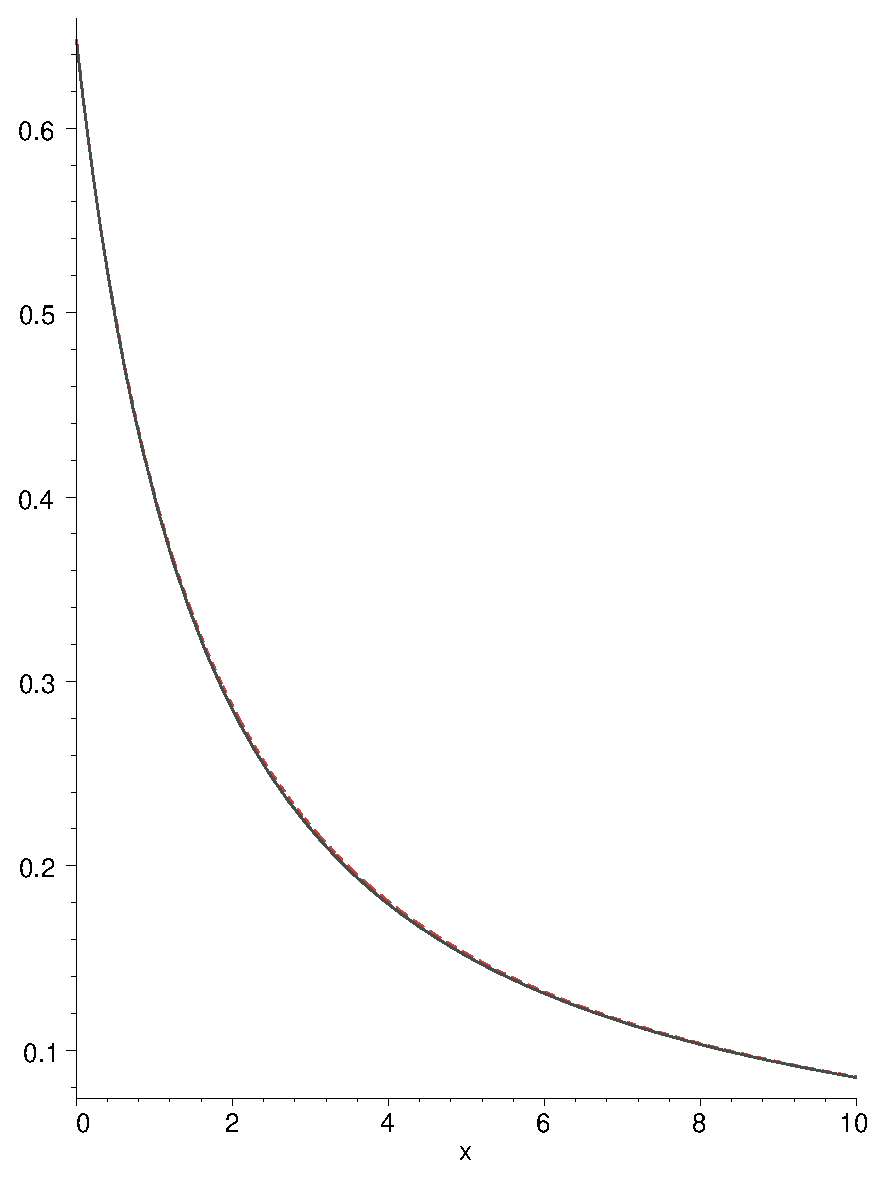
\includegraphics[  width=8cm,
  height=4cm]{winitzki01-fig01}\end{center}


\caption{A global Pad\'e approximant of degree 3 (dashed line) for the function
of Eq.~(\ref{eq:expex-fn}) (solid line).\label{fig:expex}}
\end{figure}



\subsection{Global Pad\'e approximants}

\label{sec:globalPade} Let us consider the above approximation problem
more formally. We need to approximate a function $f\left(x\right)$
which is finite everywhere in the interval $\left(0,+\infty \right)$.
Suppose that $f\left(x\right)$ has certain series expansions at $x=0$
and at $x=+\infty $,\begin{eqnarray}
f\left(x\right) & = & \sum _{k=0}^{m-1}a_{k}x^{k}+O\left(x^{m}\right)\equiv a\left(x\right)+O\left(x^{m}\right),\label{eq:fseries1}\\
f\left(x\right) & = & \sum _{k=0}^{n-1}b_{k}x^{-k}+O\left(x^{-n}\right)\equiv b\left(x^{-1}\right)+O\left(x^{-n}\right).\label{eq:fseries2}
\end{eqnarray}
Here $a\left(x\right)$ and $b\left(x\right)$ are known polynomials.
We can assume that $b_{0}=1$ in Eq.~(\ref{eq:fseries2}). We can
always reduce the problem to this case: we can divide $f\left(x\right)$
by its limit $f\left(+\infty \right)$ at $x=+\infty $ if $f\left(+\infty \neq 0\right)$.
If $f\left(+\infty \right)=0$, the series at $x=+\infty $ starts
with a higher power of $x^{-1}$ and we can multiply $f\left(x\right)$
by the appropriate power of $x$ and by a nonzero constant to make
$b_{0}=1$.

We now look for a rational approximation of the form\begin{equation}
f\left(x\right)\approx \frac{p\left(x\right)}{q\left(x\right)}\equiv \frac{p_{0}+p_{1}x+...+p_{\nu }x^{\nu }}{q_{0}+q_{1}x+...+q_{\nu }x^{\nu }},\label{eq:frat}\end{equation}
where $\nu $ is an appropriately chosen integer. The problem now
is to find the coefficients $p_{i}$, $q_{i}$ such that Eq.~(\ref{eq:frat})
has the correct expansions at $x=0$ and at $x=+\infty $. Since the
leading term of the expansion of Eq.~(\ref{eq:frat}) at $x=+\infty $
is $p_{\nu }/q_{\nu }$, we can set $p_{\nu }=q_{\nu }=1$.

This formulation is similar to the problem of Hermite-Pad\'e interpolation
with two anchor points \cite{GG99}, except that one of the points
is at infinity where we need to use an expansion in $x^{-1}$. We
call a {}``global Pad\'e approximant'' an ansatz of the form of Eq.~(\ref{eq:frat}).
The unknown coefficients $p_{i}$, $q_{i}$ are found from a system
of linear equations written compactly as\begin{eqnarray}
p\left(x\right)-q\left(x\right)a\left(x\right) & = & O\left(x^{m}\right)\textrm{ at }x=0,\label{eq:pq1}\\
\frac{p\left(x\right)}{x^{\nu }}-\frac{q\left(x\right)}{x^{\nu }}b\left(x^{-1}\right) & = & O\left(x^{-n}\right)\textrm{ at }x=+\infty .\label{eq:pq2}
\end{eqnarray}
 Here it is implied that the surviving polynomial coefficients in
$x$ or $x^{-1}$ are equated. This assumes that $p\left(x\right)$
and $q\left(x\right)$ have no common polynomial factors.

After the choice $p_{\nu }=q_{\nu }=1$, Eqs.~(\ref{eq:pq1})-(\ref{eq:pq2})
are an inhomogeneous linear system of $\left(m+n-1\right)$ equations
for $2\nu $ unknowns $p_{i}$, $q_{i}$, $0\leq i<\nu $. Therefore
a solution with lowest degree $\nu $ (when it exists) is unique if
$m+n$ is an odd number. For small degrees $\nu $ it is easy to solve
this system of equations by hand. Heuristically, the approximation
in Eq.~(\ref{eq:frat}) is the best when the orders $m$, $n$ of
expansion are close to each other, $m\approx n$.

It is important to note that the solution of Eqs.~(\ref{eq:pq1})-(\ref{eq:pq2})
with the lowest degree $\nu $ does not always exist, and when it
exists, $q\left(x\right)$ sometimes has zeros within the interval
$\left(0,+\infty \right)$. In these cases one has to choose a higher
degree $\nu $.

One can show that the construction of {}``global Pad\'e approximants''
is equivalent to Hermite-Pad\'e interpolation after a projective transformation
of the form\begin{equation}
x\rightarrow \frac{ax+b}{cx+d}.\end{equation}
Our procedure is however more direct and easier to follow in hand
calculations.


\subsection{Global approximations via identities}

The function $f\left(x\right)=\arctan x$ satisfies the identity $\frac{\pi }{2}=\arctan \frac{1}{x}+\arctan x.$
We may look for a rational function $r\left(x\right)$ that satisfies
the same identity. The simplest such function,\begin{equation}
r_{0}\left(x\right)=\frac{\pi }{2}\frac{x}{x+1},\end{equation}
approximates $\arctan x$ with absolute error $<0.06$ for all $x\geq 0$.

As another example, consider the elliptic function $\textrm{dn}\left(x,m\right)$
defined by\begin{equation}
x=\int _{\textrm{dn}\left(x,m\right)}^{1}\frac{dy}{\sqrt{\left(1-y^{2}\right)\left(y^{2}-1+m\right)}}.\end{equation}
 Here $m$ is a parameter, $0<m<1$ (we follow the conventions of
Ref.~\cite{AS64}, Chapter 16). The function $\textrm{dn}\left(x,m\right)$
is a periodic function of $x$ (on the real line) with the period
$2K$, where $K\equiv K\left(m\right)$ is the complete elliptic integral.
The function $\textrm{dn}\left(x,m\right)$ oscillates between the
minimum and the maximum values at the end points of the half-period
interval. The values of the extrema are $\textrm{dn}\left(0,m\right)=1$;
$\textrm{dn}\left(K,m\right)=\sqrt{1-m}<1$. There is a Taylor series
expansion\begin{equation}
\textrm{dn}\left(x,m\right)=1-\frac{m^{2}x^{2}}{2!}+\frac{m\left(m+4\right)x^{4}}{4!}+O\left(x^{6}\right)\label{eq:dn-taylor}\end{equation}
and an identity\begin{equation}
\textrm{dn}\left(x\textrm{,}m\right)\textrm{dn}\left(K-x,m\right)=\sqrt{1-m}.\label{eq:dn-id}\end{equation}


The obvious oscillatory approximation,\begin{equation}
\textrm{dn}\left(x,m\right)\approx \frac{1+\sqrt{1-m}}{2}+\frac{1-\sqrt{1-m}}{2}\cos \frac{\pi x}{K},\label{eq:dn0}\end{equation}
 gives about 8\% relative precision throughout the interval $x\in \left[0,K\right]$.
We can significantly improve the precision if we take into account
Eq.~(\ref{eq:dn-id}). The function\begin{equation}
r_{1}\left(x,m\right)\equiv \left(1-m\right)^{1/4}\frac{1+b\cos \left(\frac{\pi x}{K}\right)}{1-b\cos \left(\frac{\pi x}{K}\right)}\label{eq:dn1}\end{equation}
satisfies Eq.~(\ref{eq:dn-id}) for any $b$. The constant $b$ is
fixed by $r_{1}\left(0,m\right)=1$. For testing, we chose $m=0.9$
because the approximation is worst when $m$ is close to $1$. We
found that the maximum relative error of Eq.~(\ref{eq:dn1}) is less
than $10^{-4}$. 

The precision can be improved by including more cosines. For instance,
the approximant\begin{equation}
r_{2}\left(x,m\right)=\left(1-m\right)^{1/4}\frac{1+b_{1}\cos \left(\frac{\pi x}{K}\right)+b_{2}\cos \left(\frac{2\pi x}{K}\right)}{1-b_{1}\cos \left(\frac{\pi x}{K}\right)+b_{2}\cos \left(\frac{2\pi x}{K}\right)}\end{equation}
 satisfies Eq.~(\ref{eq:dn-id}), and the coefficients $b_{1,2}$
may be chosen to reproduce the first two terms of Eq.~(\ref{eq:dn-taylor}).
Then the maximum relative error of $r_{2}\left(x,m\right)$ for $m=0.9$
is less than $10^{-11}$.


\section{Global approximants for singular functions}

In this section we consider the two-point approximation problem on
the interval $\left(0,+\infty \right)$ when the function has singularities
at one or both ends of the interval.

If the function $f\left(x\right)$ has a pole at a finite $x=x_{0}$,
then we could multiply $f\left(x\right)$ by an appropriate power
of $\left(x-x_{0}\right)$ and obtain a new function without poles.
If $f\left(x\right)$ has a pole at $x=+\infty $ with the asymptotic
expansion of the form $f\left(x\right)=x^{l}\left(b_{0}+b_{1}x^{-1}+...\right)$
at $x\rightarrow +\infty $ {[}here $l>0${]}, we should select the
degree of the polynomial $q\left(x\right)$ in Eq.~(\ref{eq:frat})
to be $l$ units less than the degree of $p\left(x\right)$. Then
essentially the same procedure as above will yield a global Pad\'e approximant
for the function $f\left(x\right)$.

The presence of an essential singularity is usually clear from the
asymptotic expansion of the function $f\left(x\right)$: the expansion
contains a fractional power, an exponential, or a logarithm of $x$.
(Most often, the essential singularity is at $x=+\infty $.) It is
impossible to reproduce an exponential, a logarithmic or a power law
singularity with rational functions. Instead we should try to build
a global approximant for $f\left(x\right)$ by mixing polynomials
with the elementary functions such as $e^{x}$ or $\ln x$ in a suitable
manner. A heuristic rule that works in many cases is to write the
asymptotic at $x=+\infty $, find its other singularities, and replace
$x$ by a rational function with undetermined coefficients to remove
these singularities.


\subsection{Error function of real argument $\textrm{erf}\, x$}

The error function \begin{equation}
\textrm{erf}\, x\equiv \frac{2}{\sqrt{\pi }}\int _{0}^{x}e^{-x^{2}}dx\end{equation}
 has well-known expansions at $x=0$ and at $x=+\infty $:\begin{eqnarray}
\textrm{erf}\, x & = & \frac{2}{\sqrt{\pi }}\left(x-\frac{x^{3}}{3}+\frac{x^{5}}{10}+O\left(x^{7}\right)\right),\label{eq:erfexp1}\\
\textrm{erf}\, x & = & 1-\frac{e^{-x^{2}}}{x\sqrt{\pi }}\left[1-\frac{1}{2x^{2}}+\frac{3}{4x^{4}}+O\left(x^{-6}\right)\right].\label{eq:erfexp2}
\end{eqnarray}


A heuristic approximation may be built using the approximate identity\begin{equation}
\left(\textrm{erf}\, x\right)^{2}+\frac{\sqrt{\pi }e^{-x^{2}}}{2x}\textrm{erf}\, x\approx 1\; \Rightarrow \; \textrm{erf}\, x\approx \frac{4x}{\sqrt{\pi }e^{-x^{2}}+\sqrt{\pi e^{-2x^{2}}+16x^{2}}}\label{eq:erf-Parry}\end{equation}
(the author is grateful to Matthew Parry for bringing this to his
attention). Equation (\ref{eq:erf-Parry}) gives about 2\% of relative
precision for all real $x$. However, it is not immediately clear
how to improve the precision of this approximation.

We may transform the function $\textrm{erf}\, x$ by the ansatz\begin{equation}
\textrm{erf}\, x\equiv 1-\frac{e^{-x^{2}}}{x\sqrt{\pi }}g\left(x\right)\label{eq:erfansatz}\end{equation}
 and obtain the expansions of $g\left(x\right)$ at $x=0$ and at
$x=+\infty $,\begin{eqnarray}
g\left(x\right) & = & \sqrt{\pi }x-2x^{2}+\sqrt{\pi }x^{3}-\frac{4}{3}x^{4}+O\left(x^{5}\right),\\
g\left(x\right) & = & 1-\frac{1}{2x^{2}}+\frac{3}{4x^{4}}+O\left(x^{-6}\right).
\end{eqnarray}
The problem to approximate $g\left(x\right)$ is now in the form of
Sec.~\ref{sec:globalPade}. We may obtain, for instance, the following
global Pad\'e approximant of degree 2,\begin{equation}
g\left(x\right)\approx \frac{x\sqrt{\pi }+\left(\pi -2\right)x^{2}}{1+x\sqrt{\pi }+\left(\pi -2\right)x^{2}}.\end{equation}
 This provides a uniform approximation to $\textrm{erf}\, x$ with
an error less than $2\%$.


\subsection{Error function of imaginary argument $\textrm{erfi}\, x$}

The error function of imaginary argument $\textrm{erfi}\, x$ is defined
as $\textrm{erf}\, (ix)\equiv i\, \textrm{erfi}\, x$. The function
$\textrm{erfi}\, x$ has global approximants valid for all $x\in \left(-\infty ,+\infty \right)$,
e.g.\begin{equation}
r\left(x\right)=\frac{e^{x^{2}}}{x\sqrt{\pi }}\frac{p\left(x\right)}{q\left(x\right)},\quad \frac{p\left(x\right)}{q\left(x\right)}\equiv \frac{\frac{105}{8}x^{2}+\frac{25}{4}x^{4}+\frac{5}{8}x^{6}+x^{8}}{\frac{105}{16}+\frac{15}{2}x^{2}+\frac{9}{2}x^{4}+2x^{6}+x^{8}}.\label{eq:erfiansatz}\end{equation}
This approximates $\textrm{erfi}\, x$ to within $6\%$ of relative
accuracy for all real $x$.

Higher-order approximants may be found explicitly:\begin{eqnarray}
q_{n}\left(x\right) & = & \sum _{k=0}^{n}\frac{\left(2k-1\right)!!}{2^{k}}\left(\begin{array}{c}
 n\\
 k\end{array}
\right)x^{2n-2k},\\
p_{n}\left(x\right) & = & \sum _{l=1}^{n}x^{2l}\sum _{k=1}^{l}\frac{\left(-1\right)^{k-1}}{2^{n-l}}\frac{\left(2n-2l+2k-1\right)!!}{\left(2k-1\right)!!}\left(\begin{array}{c}
 n\\
 l-k\end{array}
\right).
\end{eqnarray}
A numerical calculation suggests that the relative error can be estimated
as\begin{equation}
\left|\frac{p_{n}\left(x\right)}{q_{n}\left(x\right)}-\textrm{erfi}\, x\right|<2^{-n}\sqrt{\frac{n}{2}}\left|\textrm{erfi}\, x\right|.\end{equation}



\subsection{The Bessel functions $J_{0}\left(x\right)$ and $Y_{0}\left(x\right)$}

A more complicated example is provided by the Bessel functions $J_{0}\left(x\right)$
and $Y_{0}\left(x\right)$. The series at $x=0$ are\begin{eqnarray*}
J_{0}\left(x\right) & = & 1-\frac{x^{2}}{4}+\frac{x^{4}}{64}+O\left(x^{6}\right)\\
Y_{0}\left(x\right) & = & \frac{2\gamma }{\pi }+\frac{2}{\pi }\ln \frac{x}{2}+\frac{x^{2}}{2\pi }\left[\gamma -1+\ln \frac{x}{2}\right]+O\left(x^{4}\ln x\right),
\end{eqnarray*}
where $\gamma \approx 0.5772$ is Euler's constant. The asymptotics
at $x=+\infty $ are\begin{eqnarray*}
J_{0}\left(x\right) & = & \sqrt{\frac{2}{\pi x}}\left(1-\frac{9x^{-2}}{128}\right)\sin \left(x+\frac{\pi }{4}\right)\\
 & + & \sqrt{\frac{2}{\pi x}}\left(-\frac{x^{-1}}{8}+\frac{75x^{-3}}{1024}\right)\cos \left(x+\frac{\pi }{4}\right)+O\left(x^{-4}\right),\\
Y_{0}\left(x\right) & = & -\sqrt{\frac{2}{\pi x}}\left(1-\frac{9x^{-2}}{128}\right)\cos \left(x+\frac{\pi }{4}\right)\\
 & + & \sqrt{\frac{2}{\pi x}}\left(-\frac{x^{-1}}{8}+\frac{75x^{-3}}{1024}\right)\sin \left(x+\frac{\pi }{4}\right)+O\left(x^{-4}\right).
\end{eqnarray*}
There are several ways to build a global ansatz that matches these
expansions. It is clear that the oscillating functions and the square
roots must be present in the ansatz. We obtained the expressions\begin{eqnarray*}
J_{0}\left(x\right) & \approx  & \sqrt{\frac{2}{\pi \left(0.123+x\right)}}\left[\sin \left(x+\frac{\pi }{4}\right)-\frac{x}{2.64+8x^{2}}\cos \left(x+\frac{\pi }{4}\right)\right],\\
Y_{0}\left(x\right) & \approx  & -\sqrt{\frac{2}{\pi \left(\frac{1}{4}+x\right)}}\left[\cos \left(x+\frac{\pi }{4}\right)+\frac{x\sin \left(x+\frac{\pi }{4}\right)}{\frac{1}{3}+8x^{2}}\right]\left(1+\frac{\ln \left(1+\frac{0.0364}{x^{2}}\right)}{2\sqrt{\pi }}\right).
\end{eqnarray*}
 {[}The constant in the argument of the logarithm is $4\exp \left(-2\gamma -2\sqrt{\pi }\right)\approx 0.0364$.{]}
These are perhaps the simplest, lowest-order global approximants accurate
away from zeros to about $2\%$ for $J_{0}\left(x\right)$ and to
about $5\%$ for $Y_{0}\left(x\right)$ for all $x\geq 0$ (see Fig.~\ref{fig:bessel0}).
Although global approximants of this kind can be found for arbitrary
orders, the (numerical) solution of the required nonlinear equations
becomes more difficult for higher orders.

%
\begin{figure}[htbp]
\begin{center}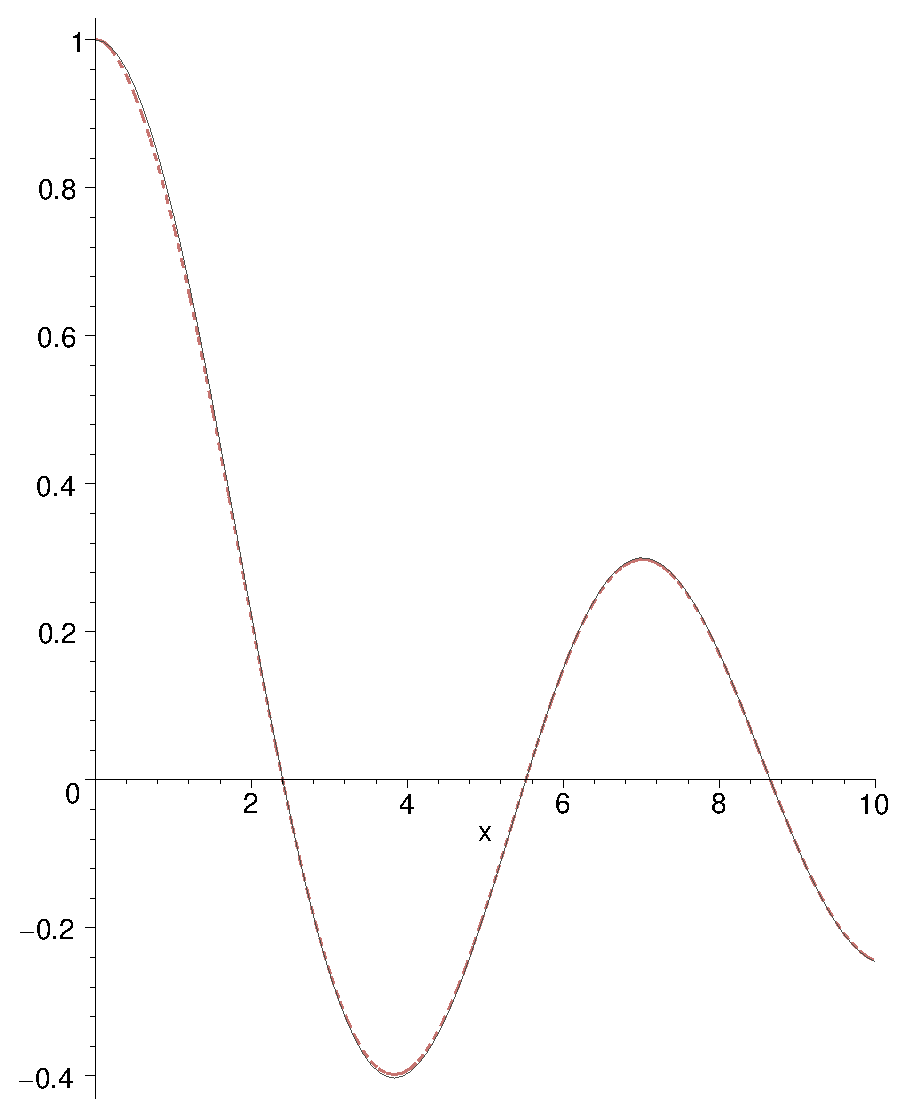
\includegraphics[  width=6cm,
  height=3.5cm]{winitzki01-fig02}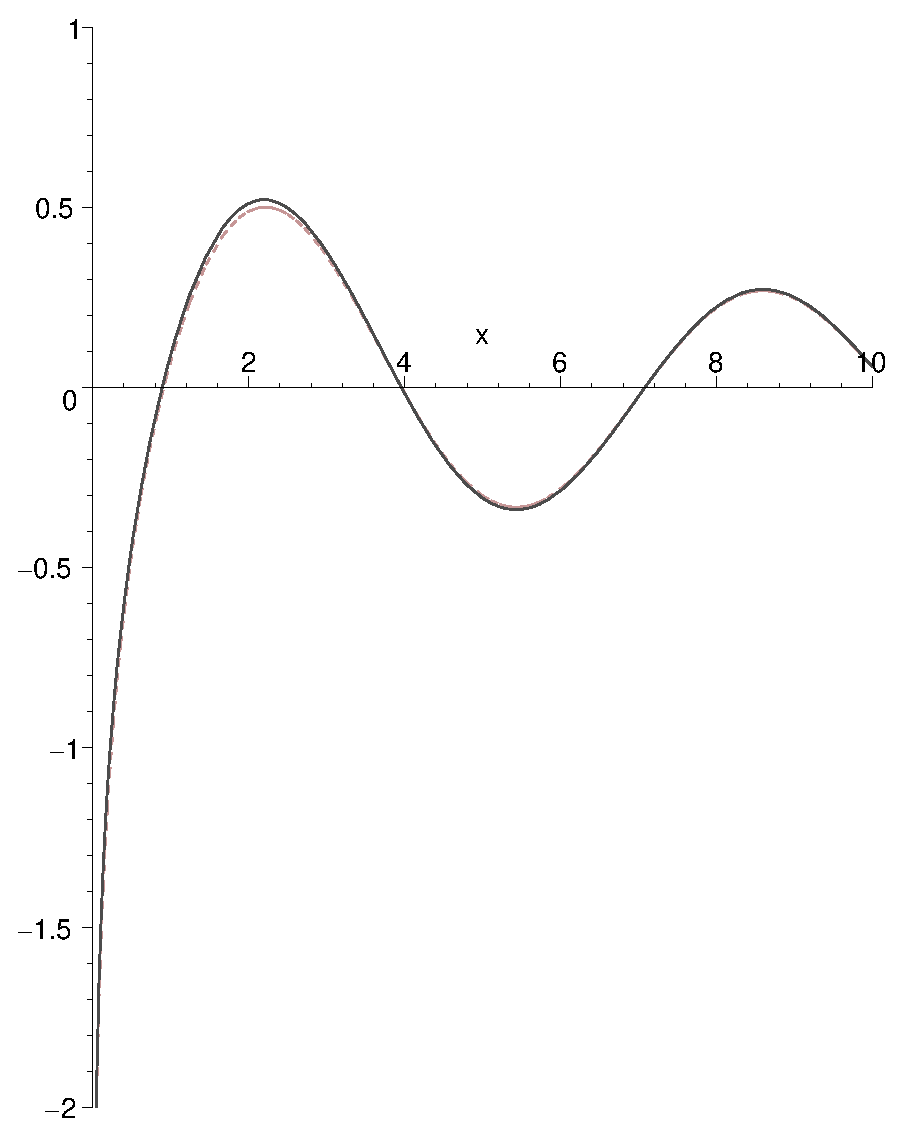
\includegraphics[  width=6cm,
  height=3.5cm]{winitzki01-fig03}\end{center}


\caption{Global approximants (dashed lines) for $J_{0}\left(x\right)$ and
$Y_{0}\left(x\right)$ (solid lines).\label{fig:bessel0}}
\end{figure}



\subsection{The Airy function $\textrm{Ai}\left(x\right)$}

The Airy function $\textrm{Ai}\left(x\right)$ has two different asymptotic
expansions at infinity,\begin{equation}
\textrm{Ai}\left(x\right)\sim \left\{ \begin{array}{l}
 \frac{1}{2\sqrt{\pi }}x^{-1/4}\exp \left(-\frac{2}{3}x^{3/2}\right)\left[1+O\left(x^{-3/2}\right)\right],\quad x\rightarrow +\infty \\
 \frac{1}{\sqrt{\pi }}x^{-1/4}\cos \left(\frac{2}{3}\left|x\right|^{3/2}-\frac{\pi }{4}\right)\left[1+O\left(x^{-3/2}\right)\right],\quad x\rightarrow -\infty \end{array}
\right.,\end{equation}
whereas the Taylor expansion at $x=0$ is\begin{equation}
\textrm{Ai}\left(x\right)=\frac{1}{3^{2/3}\Gamma \left(\frac{2}{3}\right)}-\frac{3^{1/6}\Gamma \left(\frac{2}{3}\right)}{2\pi }x+O\left(x^{3}\right).\end{equation}


It is difficult to build a single analytic ansatz for the whole real
line, and for practical purposes it is easier to approximate the Airy
function separately in the $x>0$ and $x<0$ domains. The simplest
ansatz is\begin{equation}
\textrm{Ai}\left(x\right)\approx \left\{ \begin{array}{l}
 \frac{1}{2\sqrt{\pi }}\left(x+a_{1}\right)^{-1/4}\exp \left(-\frac{2}{3}x^{3/2}\right),\quad x>0\\
 \frac{1}{\sqrt{\pi }}\left(\left|x\right|+a_{2}\right)^{-1/4}\cos \left(\frac{2}{3}\left|x\right|^{3/2}-\frac{\pi }{4}\right),\quad x<0\end{array}
\right..\label{eq:airy-1}\end{equation}
The constants $a_{1}$ and $a_{2}$ are chosen so that the value of
the ansatz at $x=0$ is correct. With the numerical values $a_{1}\approx 0.40$,
$a_{2}=4a_{1}\approx 1.60$ the ansatz of Eq.~(\ref{eq:airy-1})
approximates the Airy function to about 20\% for $x<0$ and to about
2\% for $x>0$ (see Fig.~\ref{cap:airy1}).

%
\begin{figure}[htbp]
\begin{center}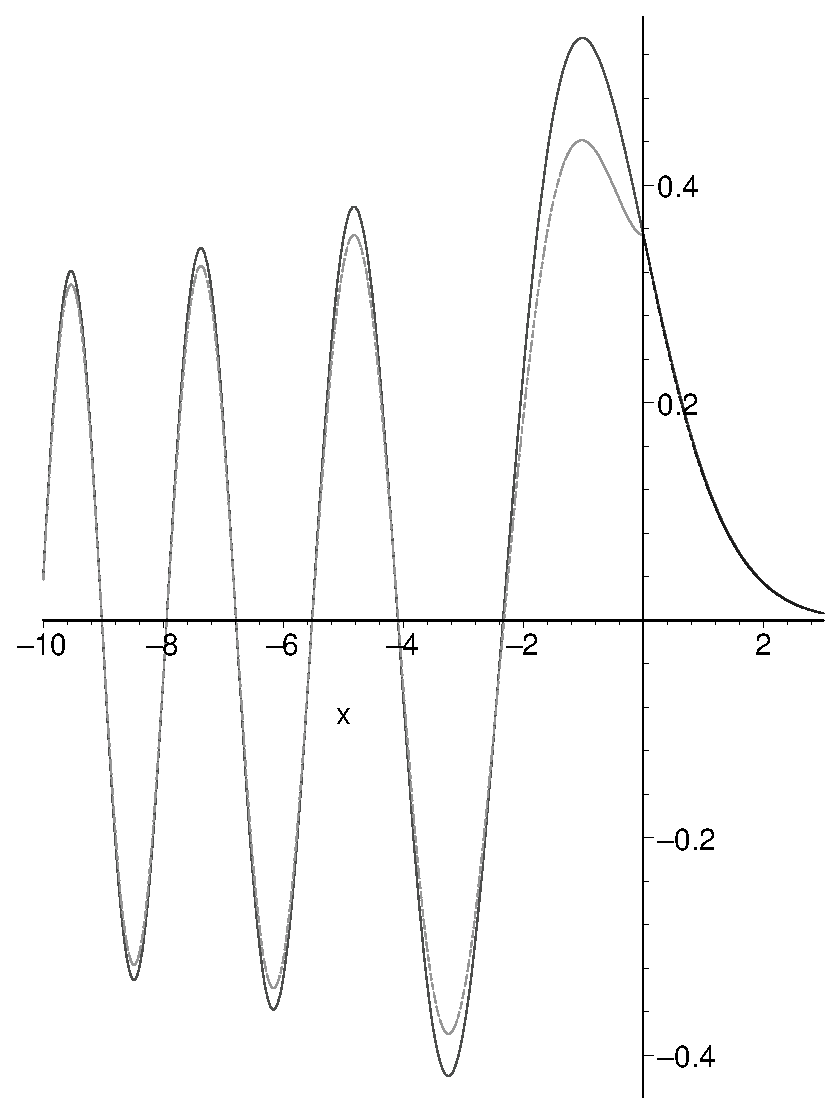
\includegraphics[  width=5cm,
  height=3.5cm]{winitzki01-fig04}\end{center}


\caption{Approximation of the Airy function $\textrm{Ai}\left(x\right)$ by
the ansatz of Eq.~(\ref{eq:airy-1}).\label{cap:airy1}}
\end{figure}


The ansatz of Eq.~(\ref{eq:airy-1}) is simple but gives a function
with a discontinuous derivative. This can be avoided with a more complicated
ansatz, for instance, replacing $\left(x+a\right)^{-1/4}$ in Eq.~(\ref{eq:airy-1})
by a more complicated function. In practice, Eq.~(\ref{eq:airy-1})
serves sufficiently well as a qualitative visualization of the Airy
function.


\subsection{Lambert's $W$ function}

Another example is Lambert's $W$ function defined by the algebraic
equation\begin{equation}
W\left(x\right)e^{W\left(x\right)}=x.\end{equation}
This function has real values for $-e^{-1}\leq x<+\infty $. We can
use the series expansions of $W\left(x\right)$ at $x=-e^{-1}$, $x=0$
and $x=+\infty $ to build global approximants on the subintervals
$\left[-e^{-1},0\right]$ and $\left(0,+\infty \right)$. The series
at $x=0$ and at $x=-e^{-1}$ are\begin{eqnarray}
W\left(x\right) & = & x-x^{2}+\frac{3}{2}x^{3}+O\left(x^{4}\right),\\
W\left(x\right) & = & -1+y-\frac{1}{3}y^{3}+\frac{11}{72}y^{4}+O\left(y^{5}\right),
\end{eqnarray}
where we defined $y\equiv \sqrt{2ex+2}$. The asymptotic expansion
at large $\left|x\right|$ is\begin{equation}
W\left(x\right)\sim \ln x-\ln \left(\ln x\right)+\frac{\ln \left(\ln x\right)}{\ln x}+\frac{1}{2}\left(\frac{\ln \left(\ln x\right)}{\ln x}\right)^{2}+...\label{eq:w1}\end{equation}


A uniform approximation for $x\in \left(0,+\infty \right)$ can be
obtained by replacing $x$ in the above asymptotic expansion by $1+x$
or other suitable rational function. For instance, the ansatz inspired
by the first three terms of Eq.~(\ref{eq:w1}),\begin{equation}
W\left(x\right)\approx \ln \left(1+x\right)\left(1-\frac{\ln \left(1+\ln \left(1+x\right)\right)}{2+\ln \left(1+x\right)}\right),\label{eq:w2}\end{equation}
approximates $W\left(x\right)$ for real $x>0$ with a relative error
less than $10^{-2}$, while\begin{equation}
W\left(x\right)\approx \frac{ex}{1+\left[\left(2ex+2\right)^{-1/2}+\frac{1}{e-1}-\frac{1}{\sqrt{2}}\right]^{-1}}\label{eq:w3}\end{equation}
is good for $-e^{-1}\leq x\leq 1$ and gives a relative error less
than $10^{-3}$.


\section{An approximation to $W\left(x\right)$ in the entire complex plane}

Here we present an approximant for $W\left(z\right)$ which is valid
for all (complex) $z$. The practical significance of a global ansatz
for $W\left(z\right)$ is to provide a precise initial approximation
$W_{0}$ for $W\left(z\right)$, from which an efficient numerical
computation of $W\left(z\right)$ for complex $z$ is possible using
e.g. the Newton-Raphson iteration.

The idea is to reproduce the first few terms of the asymptotic expansion
of $W\left(z\right)$ at large $\left|z\right|$ and of the series
at $z=0$ and at $z=-e^{-1}$. Since the expansion at $z=-e^{-1}$
uses $y\equiv \sqrt{2ez+2}$ as the expansion variable while the asymptotic
expansion uses $\ln z$, we need to combine terms of both kinds into
one ansatz. We choose an ansatz of the form\begin{equation}
W\left(z\right)\approx \frac{2\ln \left(1+By\right)-\ln \left(1+C\ln \left(1+Dy\right)\right)+E}{1+\left[2\ln \left(1+By\right)+2A\right]^{-1}}.\label{eq:Lambert-total}\end{equation}
Here the constants $A\approx 2.344$, $B\approx 0.8842$, $C\approx 0.9294$,
$D\approx 0.5106$, and $E\approx -1.213$ are determined numerically
to give approximately correct expansions at the three anchor points
to 3 terms.

Numerical computations show that Eq.~(\ref{eq:Lambert-total}) gives
the complex value of the principal branch of Lambert's $W$ function
in the entire complex plane with relative error less than $10^{-2}$,
with the standard choices of the branch cuts for $\sqrt{z}$ and $\ln z$.


\section{Conclusion}

In this paper, we have presented a heuristic method for approximating
transcendental functions $f\left(x\right)$ using combinations of
elementary functions. This method is a generalization of the Hermite-Pad\'e
interpolation to infinite intervals and non-rational functions. We
showed several examples where the approximations are easy to construct
by hand, given the first few terms of series expansions of $f\left(x\right)$
at $x=0$ and $x=+\infty $. For functions with essential singularities,
an ansatz can usually be found by replacing Laurent series and arguments
of powers and logarithms by rational functions. The simplest approximants
typically give a precision of a few percent. The numerous examples
suggest that the ansatz resulting from this procedure will approximate
the function across the entire range of the argument, $x\in \left(0,+\infty \right)$.

In one case (Lambert's $W$ function) we were able to construct a
global uniform approximant valid in the entire complex plane. This
is a somewhat surprising result; it is probably due to the simple
nature of the singularities of $W\left(z\right)$. A similar construction
will certainly be impossible for some functions such as $\Gamma \left(x\right)$
or Riemann's $\zeta \left(x\right)$ which are too ill-behaved for
a full global approximation to succeed. (However, it has been shown
that these functions allow global uniform approximants in the half-plane
domains $\textrm{Re}\, x>0$ for $\Gamma \left(x\right)$ \cite{LanczosSpouge}
and $\textrm{Re}\, x>1/2$ for $\zeta \left(x\right)$ \cite{B93};
these are the domains where these functions are free of zeros and
poles, except for the singularity at $x=+\infty $).

\begin{thebibliography}{1}
\bibitem{GG99}J. von zur Gathen and J. Gerhard, \emph{Modern Computer Algebra,}
Cambridge University Press, 1999.
\bibitem{AS64}M. Abramowitz and I. Stegun, \emph{Handbook of special functions},
National Bureau of Standards, 1964.
\bibitem{B93}P. Borwein, Canad. Math. Soc. Conf. Proc., \textbf{27} (2000), 29.
\bibitem{LanczosSpouge}C. J. Lanczos, J. SIAM of Num. Anal. Ser. B, \textbf{1} (1964), 86;
J. L. Spouge, J. SIAM of Num. Anal. \textbf{31} (1994), 931.\end{thebibliography}

\end{document}

